%%%%%%%%%%%%%%%%%%%%%%%%%%%%%%%%%%%%%%%%%%%%%%%%%%%%%%%%%%%%%%%%%%%%%%%%
%%% TODO
%%%%%%%%%%%%%%%%%%%%%%%%%%%%%%%%%%%%%%%%%%%%%%%%%%%%%%%%%%%%%%%%%%%%%%%%
%%% - Rewrite Intro
%%% - Write usb_info.tex
%%% - - Tyler Only
%%% - Write project_overview.tex
%%% - - Drafted by Monk Needs Figures
%%% - Write hardware_design_testing.tex
%%% - - Drafted by Monk Needs Figures
%%% - Write software_design_testing.tex
%%% - - Drafted by Monk Needs Figures
%%% - Write results_conclusions.tex
%%% - - Monk was last seen here
%%% - Figure out what goes in appendix
%%%%%%%%%%%%%%%%%%%%%%%%%%%%%%%%%%%%%%%%%%%%%%%%%%%%%%%%%%%%%%%%%%%%%%%%

\documentclass[12pt]{article}	% 12 pt font, report format


%\evensidemargin 0.5in % Frantically trying to fix the margin!
\usepackage[margin=1in]{geometry}

%%
%% Packages used for Thesis formating, postscript, etc.
%%
    %%
    %% Most Theses will have these:
    %%
    \usepackage{graphicx}		% Required (if you need any graphics!)
	\newcommand{\HRule}{\rule{\linewidth}{0.5mm}} % Added by Monk

    %%
    %% These packages are needed to support some of the advanced formatting
    %% options in ch_advanced.tex
    %%
    \usepackage{longtable}		% Tables longer than one page
    \usepackage{subfigure}		% Figures with sub-figures
    \usepackage[figuresright]{rotating}	% Figures & Tables sideways on page
    \usepackage{verbatim}      	        % Verbatim commands for inserting code
    \usepackage{moreverb}      	        % More of the above
    \usepackage{placeins}
    \usepackage{textcomp}

    %\LoadClass{report}
    \usepackage{float}	  		% Added by Roger
    \usepackage{listings}
    \usepackage{caption}	        % Fixes bold captions under floats
    \usepackage{url}
	\usepackage{setspace}		% Added by Monk
	\usepackage{pdfpages}		% Added by Monk

    
    %\usepackage{tocvsec2}
    
	\setcounter{totalnumber}{5}

    
    %%
    %% These packages may be helpful while writing the thesis, but should
    %% be commented out for the final version.
    %%
    %\usepackage{showkeys}	% Show the symbolic keys used for all 
    				% \label, \ref, \cite, \pageref
    
    %%
    %% The hyperref package supports document links for PDF output
    %%
%    \usepackage[colorlinks=true, 	% This should be the LAST package included
%        	pdfstartview=FitV, 	% (It my redefine or modify commands in 
%        	linkcolor=blue,		%  earlier packages)
%        	citecolor=blue, 	%
%		plainpages=false,
%		pdfpagelabels=true,
%        	urlcolor=blue]{hyperref}

%%
%% List here the files which should be recompiled on a given run.
%% For example, when writing ch2.tex, use \includeonly{ch2}
%% to compile only ch2.tex....  Latex will use the previously
%% compiled versions of all other sections to figure out pg numbers etc.
%%
\includeonly{info,body}


%%
%% Change the "senior_project_info.tex" file to have the correct title, author, etc.
%%

\begin{document}
    %%
%% Thesis Information section:
%%   Use "\\" to create a line-break for long titles
%%   \background should include the degree which is sought
%%
%%\title{Hardware and Software Solutions for Low Cost Distributed Visualization}
% Tyler please change this to something less sucky
\begin{titlepage}

\begin{center}
% Upper part of the page
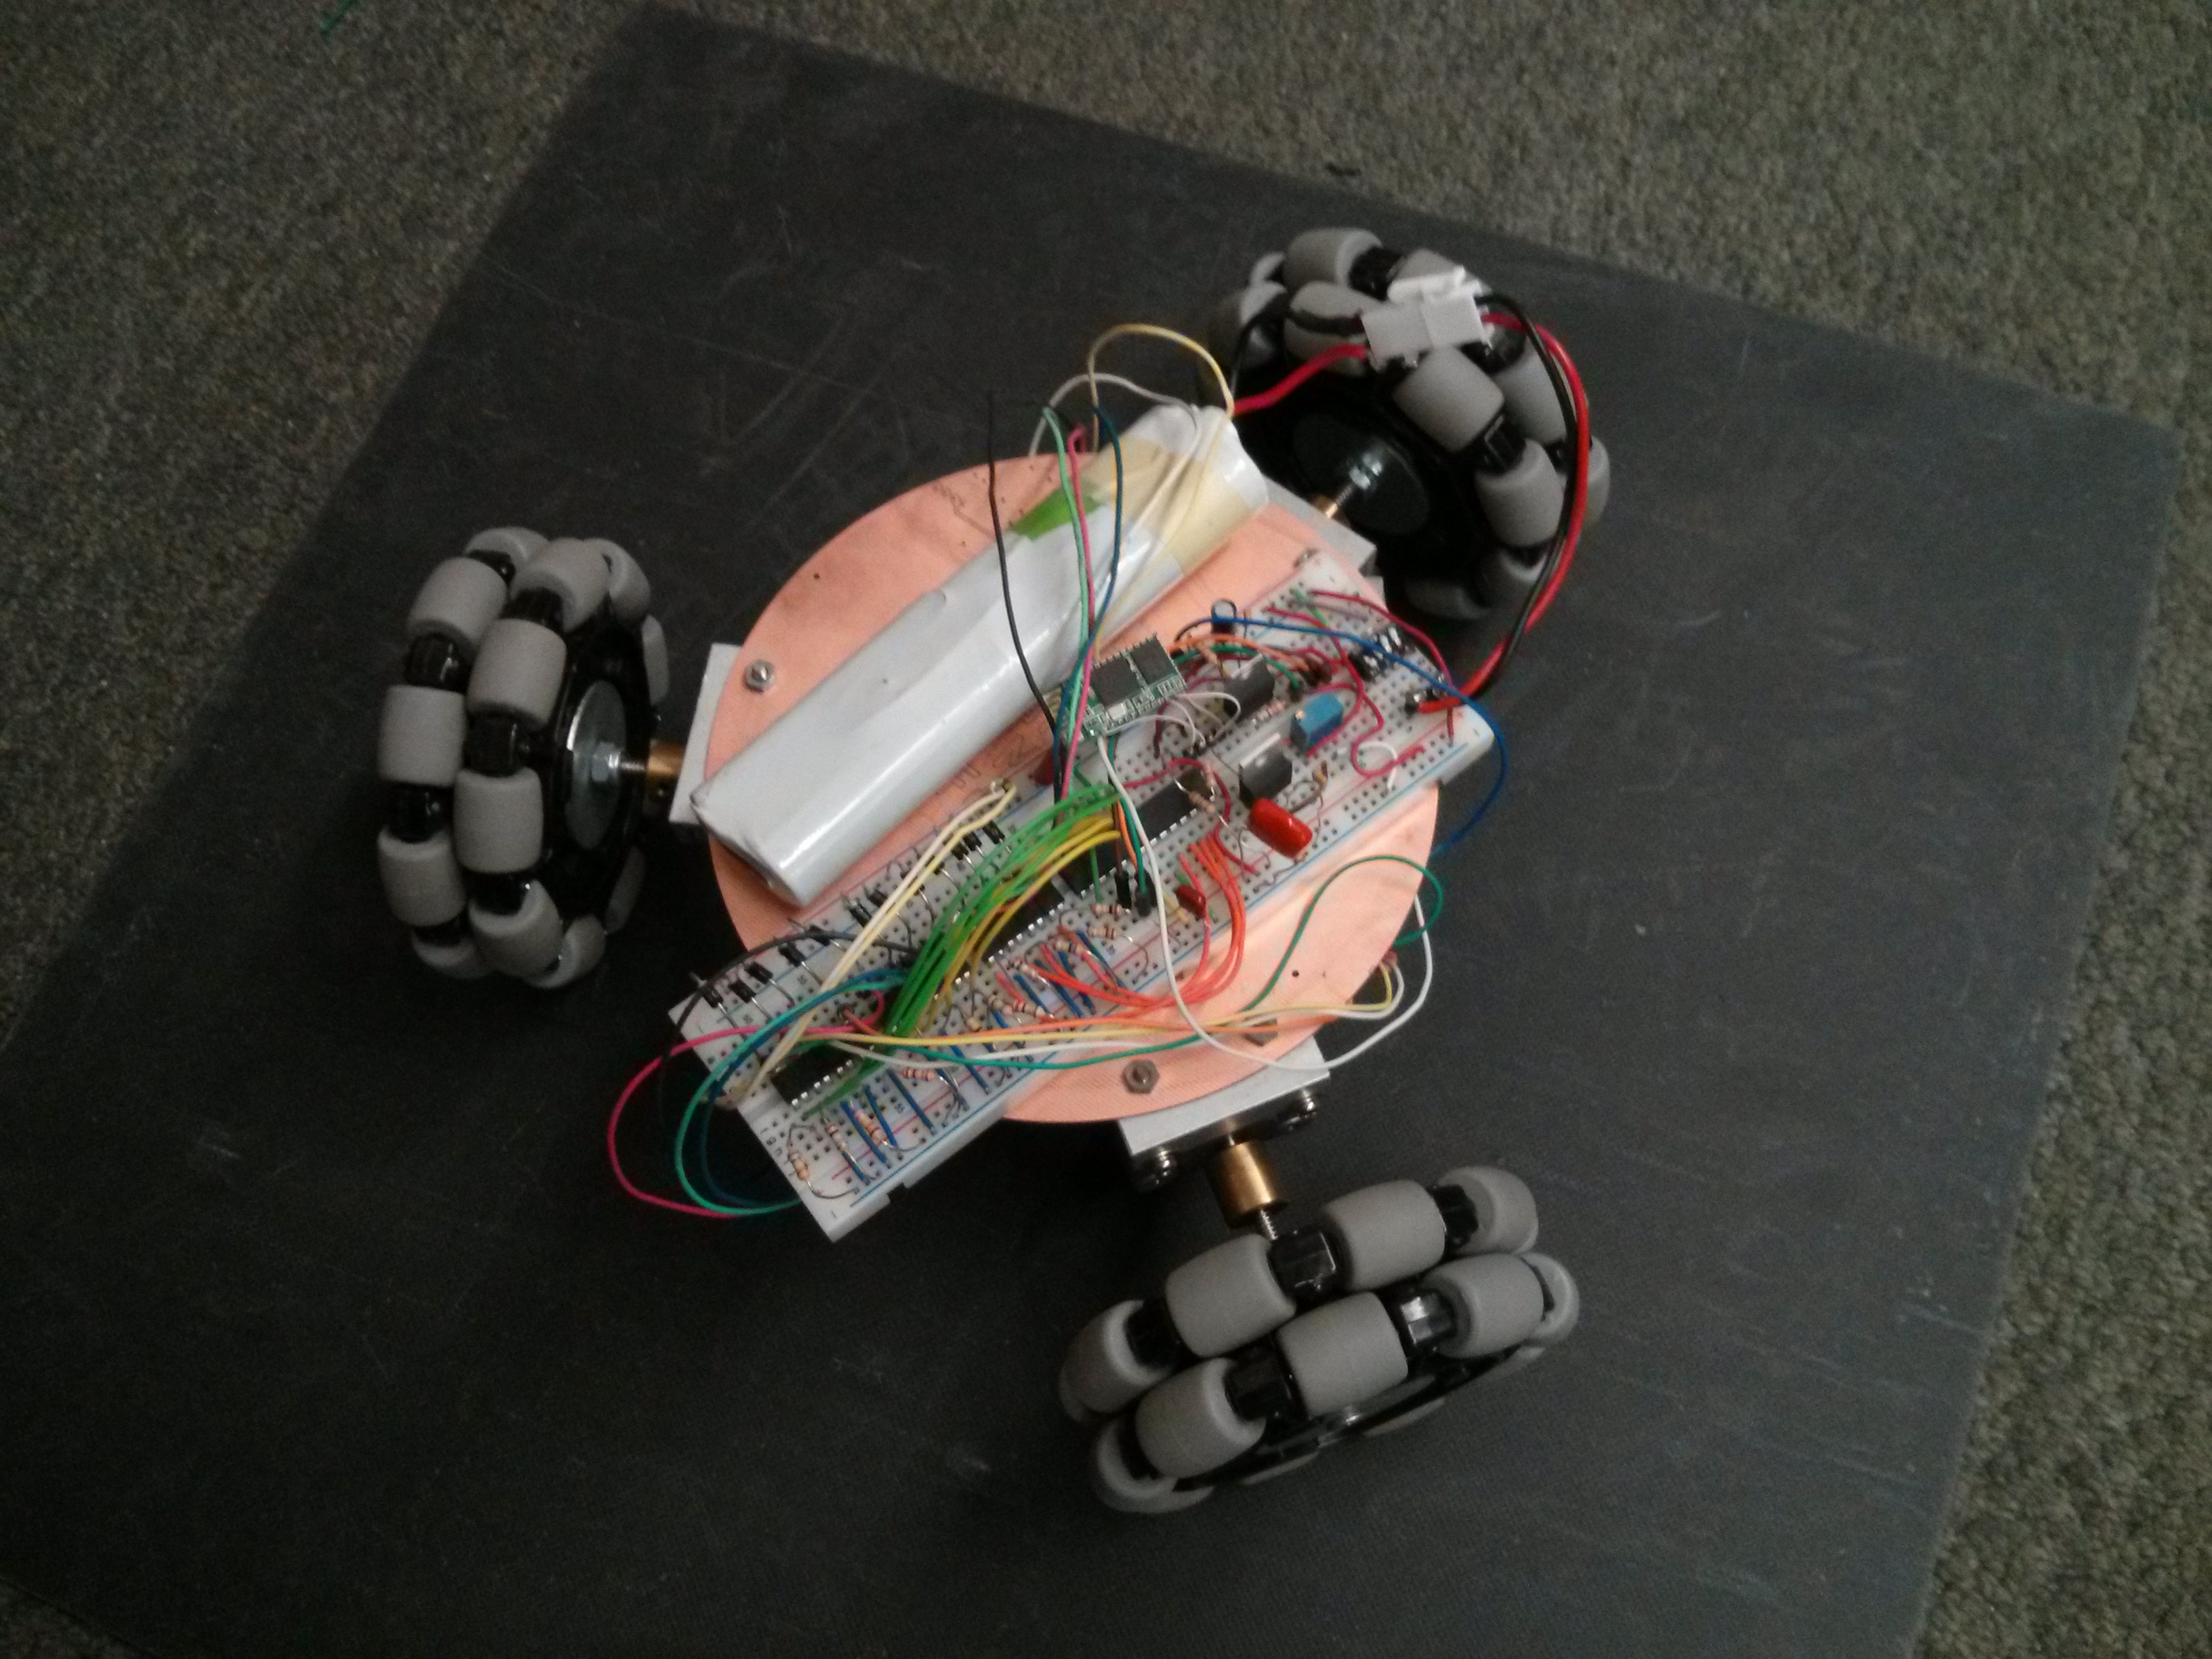
\includegraphics[width=0.6\textwidth]{./images/robot.png}
%\includegraphics[width=0.15\textwidth]{./logo}\\[1cm]    

\textsc{\LARGE }\\[1.5cm]

\textsc{\Large ECE533 Final Report}\\[0.5cm]


% Title
\HRule \\[0.4cm]
{ \LARGE \bfseries 2-Phase Unipolar Stepper\\
Omnidirectional Tri-Axis Holonomic \\
\vspace{3mm}
Drive-Train Robot}\\[0.4cm]

\HRule \\[1.5cm]

% Author and supervisor
\begin{minipage}{0.4\textwidth}
\begin{center} \large
\emph{Authors:}\\
Forrest \textsc{Flagg}\\
%\end{flushleft}
%\end{minipage}
%\begin{minipage}{0.4\textwidth}
%\begin{flushright} \large
%\emph{} \\
Aaron \textsc{McCollough}\\
%\end{flushright}
%\end{minipage}
%\begin{minipage}{0.4\textwidth}
%\begin{flushright} \large
%\emph{} \\
Jason \textsc{Monk}\\
\end{center}
\end{minipage}

\vfill

% Bottom of the page
{\large \today}

\end{center}
\end{titlepage}

    \pagestyle{empty}
    \pagenumbering{alph}

%\include{senior_project_info}
%    \maketitle

    \pagestyle{plain} 
    \pagenumbering{roman}



%%     {\singlespacing
%% 	\pdfbookmark[0]{TABLE OF CONTENTS}{my_toc}
% 	\tableofcontents
% 	\listoftables
% 	\listoffigures
     \newpage \pagenumbering{arabic}
%    \pdfbookmark[0]{TABLE OF CONTENTS}{my_toc}

    %\let\myNumberline\numberline    % required to add Table and Figure text
    %                                % to lof and lot
    %\tableofcontents
    %\renewcommand\numberline[1]{\myNumberline{Table #1:}}  % add "Table" text as required by grad school
    %\listoftables
    %\renewcommand\numberline[1]{\myNumberline{Figure #1:}} % add "Figure" text as required by grad school
    %\listoffigures
    %\renewcommand\numberline[1]{\myNumberline{#1}} % restore \numberline to the starting definition.
    %} 
    %\addtocontents{toc}{\protect{\vspace{1.5\baselineskip} \noindent Chapter}}
    %\newpage \pagenumbering{arabic}

	\onehalfspacing
    \section{Introduction}

The field of robotics is rapidly expanding as new and different robots are created to perform a variety of tasks. Many robots employ various locomotion techniques for navigation, the most popular of which is a four wheel, two axis setup. This works great for many applications but has some drawbacks when trying to perform complicated maneuvers. This is where the omnidirectional, holonomic drive train comes in. By employing three omni wheels on three individually controlled drive shafts, a holonomic drivetrain enables the robot to at once move in any direction and rotate in place without having to change it’s orientation. This is a huge improvement over conventional 4 wheeled robots. This remarkable drive system was the inspiration for this project and the reason we chose to build a 2-Phase Unipolar Stepper Omnidirectional Tri-Axis Holonomic Drive-Train Robot.

\section{Circuit}

The figure below shows the schematic for the board.

\begin{figure}[H]
    \begin{center}
        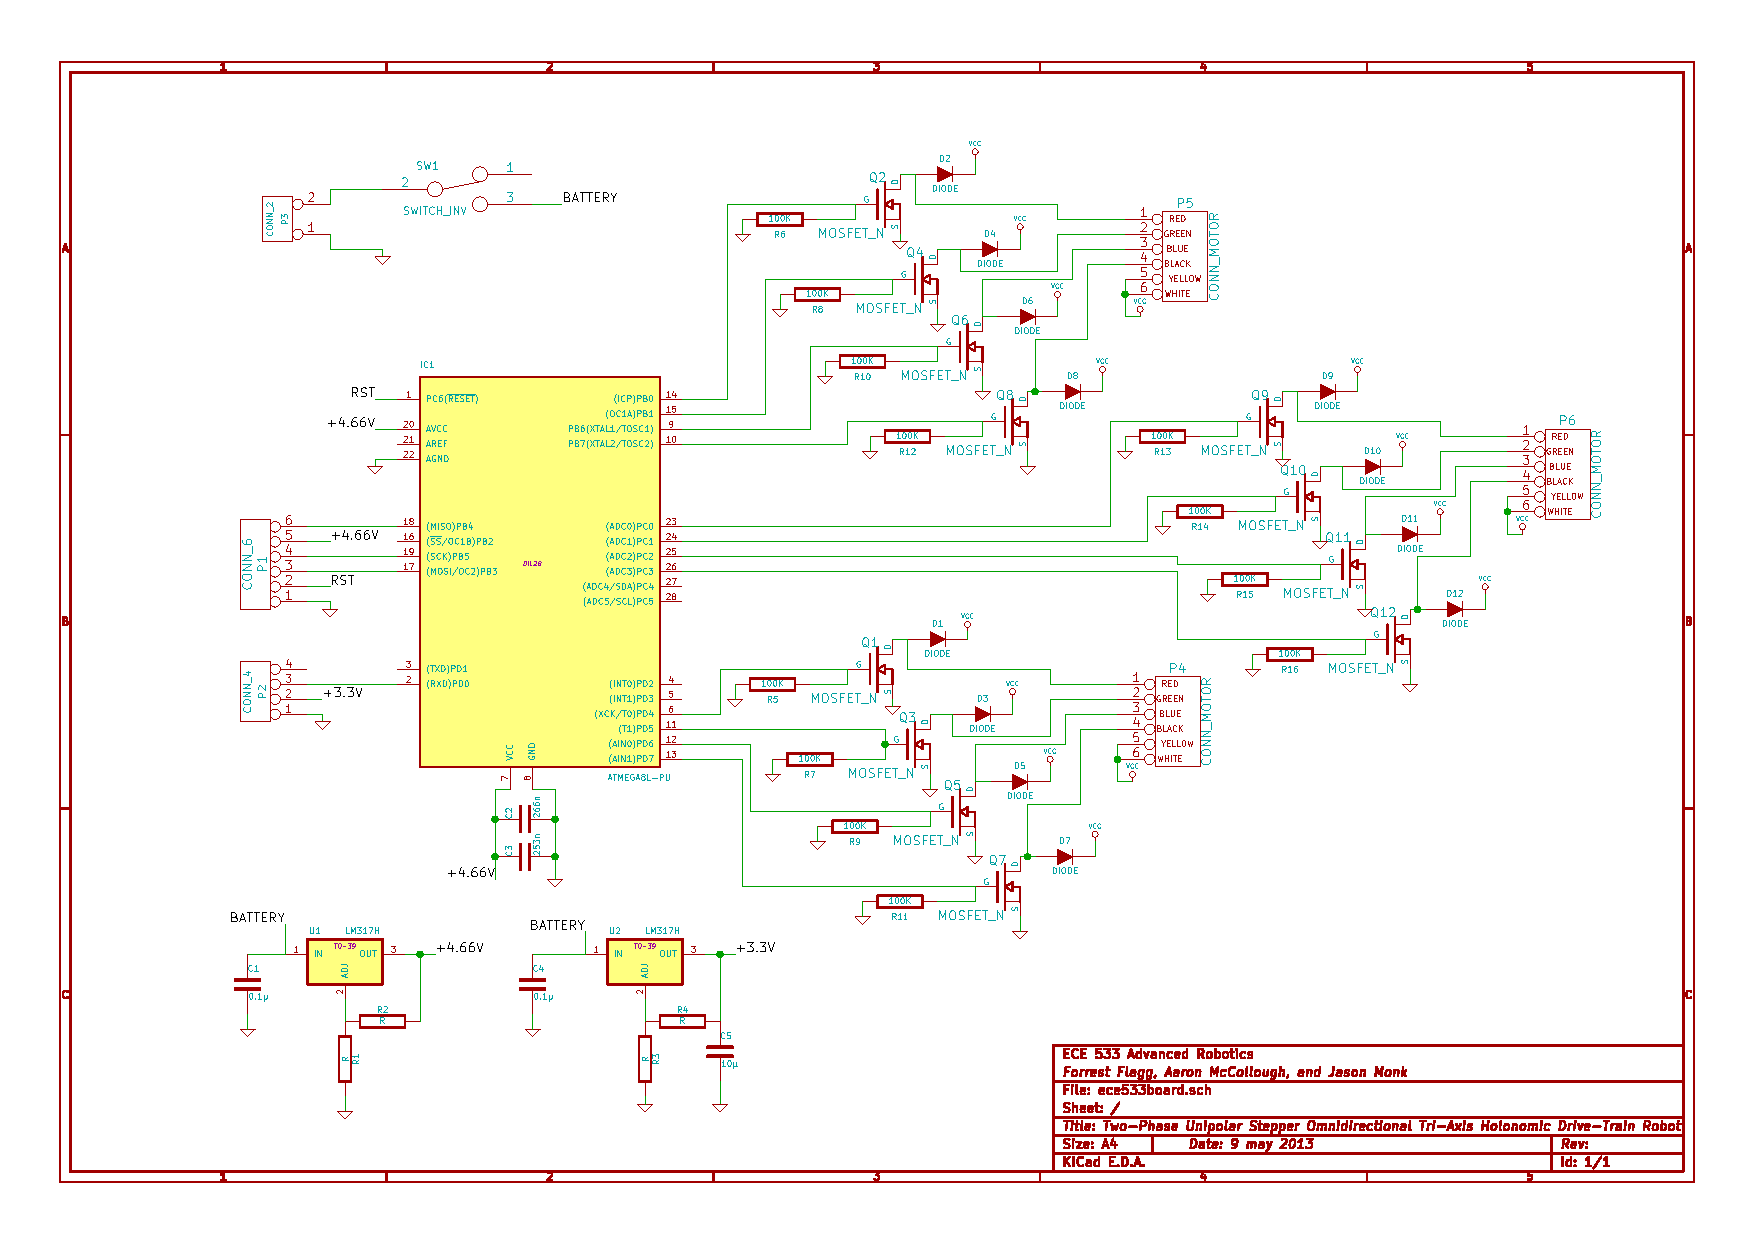
\includegraphics[width=.99\textwidth]{images/ece533board.eps}
    \end{center}
    \caption{Full Schematic}
    \label{figure:schematic}
\end{figure}

The microprocessor that drives the robot is an ATmega8L.  This chip is a 28 pin PDIP package.  The ATmega8L can run at up to 8MHz which is currently being used.  It has 8kB of programmable flash memory and 1kB of internal SRAM and can run on voltages between 2.7V and 5.5V.

The MOSFETs which drive the motors are IRFD110.  The Vgs specification for these MOSFETs is minimum 2V and maximum 4V.  They are driven at 4.66V on the robot to ensure full saturation and allow maximum torque for the motors.

Two voltage regulators are used to supply the three voltage levels needed.  The regulators are LM317 linear adjustable voltage regulators.  One supplies the 3.3V line that powers the Bluetooth chip and the other supplies the 4.66V rail which runs the microprocessor.

The Bluetooth communication chip is designed to be a drop in replacement for serial communication lines.  Only three pins are needed It runs at 3.3V and is specified to run at up to 5.6V, but communication fails not far above 3.3V.

The stepper motors are described in Section \ref{section:stepper}.

The batteries that power the robot are 7.4V 5200mAh Li-ion rechargeable batteries made by Powerizer.

\section{Stepper-Motor Driving}
\label{section:stepper}

A stepper motor is a type of DC electric motor that operates by energizing an electromagnet to pull the motor into a specific position.  Several electromagnets are arranged so that when energized in sequence the motor will move forward, and the reverse sequence moves it backwards.

The motors being used are PX-245-2B-C8 (AKA 101 Motors).  These are Uni-polar stepper motors, which have several types of driving methods.  Figure \ref{figure:driving} shows the common driving modes for this type of stepper motor.

\begin{figure}[H]
    \begin{center}
        \includegraphics[width=3in]{images/Drive.png}
    \end{center}
    \caption{Unipolar Driving Modes from Wikipedia}
    \label{figure:driving}
\end{figure}

With the hardware setup described in Section \ref{section:hardware}, we are capable of achieve Wave, Full Step and Half Step Drives.  In testing we achieved the greatest torque from the motors from the Half Step Driving pattern, so that is what is currently implemented.

\subsection{Hardware}
\label{section:hardware}

As shown in the schematic, there is a driver for each of the coils on all of the motors.  The motor is driven by connecting one side of the coil to Vcc and the other to a driving MOSFET (IRFD110).  The MOSFET is turned on to energize that coil in the motor.  Since the motors are primarily inductive, diodes (1N4004) allow the current to feedback into the Vcc rail when the coil is turned off.

\subsection{Software}

To control all three stepper motors a fair amount of asynchronous structure was required in the code.  The first step was to setup a timer interrupt that ran at 10 KHz.  This interrupt checks if each of the motors needs updating.  It does this by decrementing 3 counters and updating motor values when its respective counter reaches zero, then reseting the counter to the top.  When a motor is updated a flag is set to indicate a new motor state is required to be calculated.  There is a fourth counter which is used for timing when doing automated testing (i.e. going in a circle).

\begin{figure}[H]
\begin{lstlisting}
ISR(TIMER1_COMPA_vect) {
    TCNT1 = 0;
    if (--counter1 == 0) {
        PORT_1 = motorState1;
        needState1 = TRUE;
        counter1 = speed1;
    }
    if (--counter2 == 0) {
        PORT_2 = motorState2;
        needState2 = TRUE;
        counter2 = speed2;
    }
    if (--counter3 == 0) {
        PORT_3 = motorState3;
        needState3 = TRUE;
        counter3 = speed3;
    }
    if (--counter4 == 0) {
        needsNewSpeed = TRUE;
        counter4 = speed4;
    }
}
\end{lstlisting}
\caption{AVR Timer Interrupt Handler}
\label{figure:interrupt}
\end{figure}

When the needState flags are set the main code calculates the next motor state to be queued for output.  The next state calculated the same way for each of the motors, either moving forward or backward in the stepping sequence, but the calculation of the port value varies for each of the motors because they reside in different areas of the port.

\begin{figure}[H]
\lstset{tabsize=4}
\begin{lstlisting}
while (1) {
	...
	if (needState1) {
		currentState1 = getNextState(currentState1, movingForward1);
		motorState1 = getMotorState(currentState1);
		needState1 = FALSE;
	}
	if (needState2) {
		currentState2 = getNextState(currentState2, movingForward2);
		motorState2 = getMotorState(currentState2) << 4;
		needState2 = FALSE;
	}
	if (needState3) {
		currentState3 = getNextState(currentState3, movingForward3);
		state = getMotorState(currentState3);
		motorState3 = ((state & 0x0C) << 4) | (state & 0x03);
		needState3 = FALSE;
	}
}
\end{lstlisting}
\caption{Next State Calculation}
\label{figure:next_state}
\end{figure}

The states of the motor are stored in a buffer that can easily be changed to any of the motor driving techniques described above.  Then the motor states can be traversed by moving forward or backward through the state array;

\begin{figure}[H]
\begin{lstlisting}
const unsigned char motorStates[8] = 
        {0x01, 0x03, 0x02, 0x06, 
         0x04, 0x0C, 0x08, 0x09};

unsigned char getMotorState(unsigned char state) {
    return motorStates[(int)(state & 0x07)];
}
\end{lstlisting}
\caption{Next State Function}
\label{figure:next_state_func}
\end{figure}

A simple helper function controls the movement between states based on the current state and the direction of the motor.  It performs an increment or decrement modulo 8.

\begin{figure}[H]
\begin{lstlisting}
unsigned char getNextState(unsigned char currentState, 
                           unsigned char movingForward) {
    if (movingForward) {
        ++currentState;
    } else {
        --currentState;
    }
    return currentState & 7;
}
\end{lstlisting}
\caption{Next State Iteration}
\label{figure:next_state_iter}
\end{figure}


\section{Omni-Directional Control}



When moving the robot there are two aspects that need to be considered. The translation component and the rotation component. These actions can be considered separately and then combined after the calculations have been made. There are some caveats to this and they will be discussed in the following sections. 

\subsection{Translation Component}

The basic kinematics for each wheel on the robot can be shown in figure \ref{figure:kinematics}. The direction vector shown indicates the direction the robot wants to go relative to the wheel. The speed at which the wheel must turn is proportional to the component of that vector that lies perpendicular to the wheel’s axis, indicated by the red arrow. The wheel magnitude vector can be calculated as shown in the following equation:

\begin{equation}
S = V * \sin (\Theta) .
\end{equation}

Where S is the wheel speed and V is velocity of the robot.


\begin{figure}[H]
    \begin{center}
        \includegraphics[width=3in]{images/motion_control.png}
    \end{center}
    \caption{Wheel Kinematics Diagram}
    \label{figure:kinematics}
\end{figure}

To calculate the wheel magnitude vector for the other two wheels, simply add an offset of 120 degrees and 240 degrees respectively to the direction vector angle.

\subsection{Rotation component}

The rotation component is much simpler than the translation component. If you want the robot to rotate in one direction simply run all the wheels in the same direction at the same speed. If the speeds are different the robot will still rotate but there will be some translation as well.

\subsection{Combining Translation and Rotation}

If you want the robot to move some distance and rotate some number of degrees at the same time you can simply calculate the translation and rotation components separately and then sum the results for each wheel. Setting the wheels to this speed will cause the robot to move that distance and rotate that amount but the result of rotating while translating is that the robot will veer off course. This is because the translation is relative to the orientation of the robot and if that orientation is changing so will the direction of the robot.

One solution is to constantly update the robot wheel speeds to accurately reflect the position and orientation of the robot in it’s current time step so that even as it’s rotating the translation calculations are being made based on the robots current angle and not the start angle. This solution is not ideal because it requires many, rapid, updates. In the ideal case it would require an infinite amount of updates. Our solution is to find a translation vector and a rotation speed that can be set to move the robot from any position and orientation to any other with a non-changing wheel speed.

For this to work the robot will have to travel in an arc from one point to the next. The length of the arc is derived from the law of cosines and is given in the following equation:

\begin{equation}
D = \sqrt{\frac{\Delta x^2 \times \Delta y^2}{2 - 2 \cos (\Theta)}} \times \Theta.
\end{equation}

The translation angle of the robot is given by:

\begin{equation}
\Theta_s = \arctan (\frac {\Delta x} {\Delta y} ) + \frac {\Theta_r} {2}.
\end{equation}

Now that we know the distance the robot must travel we can calculate the time that a given operation will take.

\begin{equation}
Time = \frac {D} {S}.
\end{equation}

The rotation component of the robot can now be calculated.

\begin{equation}
\phi = \frac {\Theta_r} {Time}.
\end{equation}

Now that the adjusted translation component and the rotation component are known they can be combined to give each wheel’s individual speed to control the robot.


\begin{figure}[H]
\begin{lstlisting}
//relative new x and y
float x = rloc.x;
float y = rloc.y;
//relative rotation in radians
float rot = rloc.rot;
Log.e("ROBOT PATH", "L: " + x + " " + y + " Rot: " + rot);

//finalant variables
//Robot radius
final float robot_rad = 4.75f;
//Wheel radius;
final float wheel_rad = 2.0f;
//Maximum Robot Speed
final float max_speed = 6.28f;

float radius,d,fulld;

// linear distance to next point
d = (float) Math.sqrt(x*x + y*y);

// radius of circle that the arc lies on
radius = (float) Math.sqrt(d*d/(2*(1-Math.cos(rot))));

// length of the arc
fulld = radius*Math.abs(rot);

//start_rot = rot/2;
double final_angle = Math.atan2(y,x) + rot/2;

// calculate the time to next state
float time = fulld/max_speed;
double rob_rot = rot * robot_rad / (/*2 * */wheel_rad) / time;
Log.e("ROBOT PATH", "Rotation: " + rob_rot);

// Calculate ticks per second
double tps1 = (Math.sin(final_angle)*max_speed * 1/2 + rob_rot) 
										* (180/(0.9*Math.PI));
double tps2 = (Math.sin(final_angle+RobotControl.off2)*
                              max_speed * 1/2 + rob_rot) 
                                        * (180/(0.9*Math.PI));
double tps3 = (Math.sin(final_angle+RobotControl.off3)*
                              max_speed * 1/2 + rob_rot) 
                                        * (180/(0.9*Math.PI));
\end{lstlisting}
\caption{Control Implementation}
\label{figure:robot_math}
\end{figure}

\section{Wireless Communication}

We wanted the robot to be completely wireless as its omni-directional nature is not exactly condusive to having any wires hanging off from it.  The robot currently uses a bluetooth transciever to communicate with phones or computers.

\subsection{Bluetooth}
\label{section:bluetooth}

The Bluetooth communication chip has a number of features that are not being utilized.  The chip supports interfaces for USB, UART, SPI, and PCM.  Only the UART interface is currently used.  This allows the chip to be a transparent replacement for serial UART lines.  The chip handles all of the Bluetooth communication including pairing, the Bluetooth stack, and pin security. 

\begin{figure}[H]
    \begin{center}
        \includegraphics[width=2in]{images/bluetooth.png}
    \end{center}
    \caption{Bluetooth Device Used}
    \label{figure:bluetooth}
\end{figure}

\subsection{Protocol}

The communication from the AVR side is extremely simple.  The AVR recieves data on the UART at 9600 Baud.  At the top of every main loop the code checks for incoming serial communication and stores it in the buffer.  When it has received 6 bytes it interprets them as 3 signed integer values, these are then used as delays for each of the motor driving. 

\begin{figure}[H]
\begin{lstlisting}
char index = 0;
int speeds[3];
char* buffer = (char*) speeds;

while (1) {
    if  (UCSRA & (1<<RXC)) {
            buffer[index++] = UDR;

            if (index == 6) {
                    setSpeed1(speeds[0]);
                    setSpeed2(speeds[1]);
                    setSpeed3(speeds[2]);
                    index = 0;
            }
    }
	...
}
\end{lstlisting}
\caption{Serial Receive}
\label{figure:uart_receive}
\end{figure}

The setSpeed function simply handles the signed number so that positive goes forward and negative goes backwards.

\subsection{Android}
\label{section:android_wireless}

To connect to the bluetooth chip on android some complicated code was required.  Figure \ref{figure:android_bluetooth} shows the code that connects to the bluetooth chip described in Section \ref{section:bluetooth}.  It uses reflection to access the function createRfcommSocket, which is no longer available in current android APIs.  The code then calls the function on the device which opens a socket communication with it.

\begin{figure}[H]
\begin{lstlisting}
// hard coded the MAC of our bluetooth chip
device = adapter.getRemoteDevice("00:19:5D:EE:08:05");

// breaks out functions that are no longer broken out for our use
// specifically connect
Method m = device.getClass().getMethod("createRfcommSocket",
		new Class[] { int.class });
bluetoothSocket = (BluetoothSocket) m.invoke(device, 1);

// connect to the board
bluetoothSocket.connect();
\end{lstlisting}
\caption{Android Bluetooth Connection}
\label{figure:android_bluetooth}
\end{figure}

In practice we had a lot of reliability issues with using Android to connect to this bluetooth device.  It would sometimes have problems disconnecting, then problems reconnecting, and required rebooting the phone a lot.  The workaround used for this was to use a laptop to connect to the bluetooth device, then use a socket forwarding program (socat).

\begin{figure}[H]
    \framebox[\textwidth][s]{
            \parbox{\linewidth}{
\$ sudo rfcomm connect rfcomm0 00:19:5D:EE:08:05 \\
\$ sudo socat TCP-LISTEN:8023,fork /dev/rfcomm0,raw,b9600,echo=0
}}
\caption{Socket Forwarding}
\label{figure:socket_forwarding}
\end{figure}

\section{Android App}

An Android App was developed to control the robot.  There are two modes of control that were supported.  The first is referred to as Simple Control and allows the user to direct the robot to move in any direction or turn in any direction.  The second mode is referred to as Fancy Control and utilizes multitouch to allow the user to draw a path and orientation for the robot to move.

Figure \ref{figure:menu} shows the startup screen for the app.  It allows the user to enter either of the modes above.  It also allows the user to set the IP for the Socket-Bluetooth bridge as discussed in Section \ref{section:android_wireless}.

\begin{figure}[H]
    \begin{center}
        \includegraphics[width=2in]{images/menu.png}
    \end{center}
    \caption{Android App Main Menu}
    \label{figure:menu}
\end{figure}

Figure \ref{figure:host_control} shows an example of setting the IP and Port of the Socket-Bluetooth bridge.

\begin{figure}[H]
    \begin{center}
        \includegraphics[width=2in]{images/host_control.png}
    \end{center}
    \caption{Android host Selection}
    \label{figure:host_control}
\end{figure}

\subsection{Surface View}

Both the Simple and Fancy Control use a Surface View to have direct control to drawing on the screen.  The Surface View creates a Surface Holder which allows access to the canvas for the screen.  Figure \ref{figure:canvas_renderer} shows how the rendering thread gets the canvas from the surface holder.

\begin{figure}[H]
\begin{lstlisting}
public void run() {
	long lastTime;
	while (mRun) {
		lastTime = System.currentTimeMillis();
		if (holder != null) {
			canvas = holder.lockCanvas();
			if (canvas != null) {
				drawFrame();
				holder.unlockCanvasAndPost(canvas);
			}
		}
		
		long diff = delay - (System.currentTimeMillis() - lastTime);
		try {
			if (diff > 0) {
				sleep(delay);
			}
		} catch (InterruptedException e) {
			e.printStackTrace();
		}
	}
}
\end{lstlisting}
\caption{Socket Forwarding}
\label{figure:canvas_renderer}
\end{figure}

The function drawFrame varies from Simple to Fancy control but both of them use the canvas created to draw directly onto the screen.

\subsection{Multitouch Control}

Handling multitouch on android is a fairly simple process.  Whenever the Current Activity receives a onMotionEvent call, the Activity passes it off to a class to track the location of all fingers on the screen.

\begin{figure}[H]
\begin{lstlisting}
public void updateTouch(MotionEvent event) {
	if (isMultitouch) {
	    final int pointerCount = event.getPointerCount();
	    for (int i = 0; i < pointerCount; i++) {
            final int action = event.getAction();
            final int actual = action & MotionEvent.ACTION_MASK;
            final int id = event.getPointerId(i);
            if (actual == MotionEvent.ACTION_POINTER_UP || 
                        actual == MotionEvent.ACTION_UP || 
                        actual == MotionEvent.ACTION_CANCEL) {
            	unTouch(id);
            } else {
            	touch(id, event.getX(i), event.getY(i));
            }
	    }
	} else {
		if (event.getAction() == MotionEvent.ACTION_UP) {
			unTouch(0);
		} else {
			touch(0, event.getRawX(), event.getRawY());
		}
	}
}
\end{lstlisting}
\caption{MultiTouch Tracking}
\label{figure:android_multitouch}
\end{figure}

\subsection{Simple Control}

The simple controller draws a circle and a bar on the screen.  It then looks for touches within the circle or the bar.  When a touch is within the circle it moves the robot in the direction from the center of the circle to the finger, at a speed proportional to the distance from the center.  The bar performs similarly except it controls the rotation of the robot and only operating on the X axis.

\begin{figure}[H]
    \begin{center}
        \includegraphics[width=2in]{images/simple_control.png}
    \end{center}
    \caption{Android Simple Control Interface}
    \label{figure:simple_control}
\end{figure}

The bottom of the screen shows true/false indicating whether the app has successfully connected to the TCP Socket/Bluetooth.  This can help significanty when debugging the connection to the robot.

\subsection{Fancy Control}

The Fancy Controller has a much simpler display to it.  It draws a blue background to draw on,  red dots for each of the fingers detected by multitouch, and the path that has been detected so far.  Figure \ref{figure:fancy_control} shows the display with all three of these in effect.

\begin{figure}[H]
    \begin{center}
        \includegraphics[width=2in]{images/fancy_control.png}
    \end{center}
    \caption{Android Fance Control Interface}
    \label{figure:fancy_control}
\end{figure}

The path is created by sampling the finger locations every 1/4th second.  When there are 2 fingers on the screen the path is recorded.  The path is interpreted as the point half way between the fingers being the desired robot location, and the angle of the vector between them as being the position.  The point at which the fingers are set down on the screen is assumed to be (0, 0, 0), which is the current position of the robot.  When the number of fingers on the screen changes to anything besides 2 the path for the robot is calculated and the robot follows it.  Figure \ref{figure:android_tracking} shows the code that gets called every 1/4th second to check the number of fingers/locations of those fingers.

\begin{figure}[H]
\lstset{tabsize=2}
\begin{lstlisting}
private void updatelocations() {
	int numactive = 0;
	Location l1 = null;
	Location l2 = null;
	Point point;
	for (int i = 0; i < TouchController.MAX_POINTS; ++i) {
		point = touchcontroller.getPoint(i);
		if (point.isSet()) {
			++numactive;
			if (l1 == null) {
				l1 = new Location(point.getX(), point.getY());
			} else {
				l2 = new Location(point.getX(), point.getY());
			}
		}
	}
	synchronized (locs) {
		if (isupdating) {
			if (numactive != 2) {
				isupdating = false;
				path = new RobotPath(locs, TouchActivity.robotControl);
				path.start();
			} else {
				if (Math.max(l1.dist(locs.get(locs.size() - 1).first), 
                             l2.dist(locs.get(locs.size() - 1).second)) 
                             > THRESH) {
					locs.add(new Pair<Location, Location>(l1, l2));
				}
			}
		} else {
			if (numactive == 2) {
				locs.clear();
				locs.add(new Pair<Location, Location>(l1, l2));
				isupdating = true;
			}
		}
	}
}
\end{lstlisting}
\caption{Finger Tracking}
\label{figure:android_tracking}
\end{figure}

\section{Future Work}

This project has a number of ways in which it could be improved in the future.  This section details a few that we have thought about and partially explored, and how we think they could help out the robot.

\subsection{Protocol}
The current protocol allows for a fair amount of error to occur.  When the information being sent is offset by 2 bytes then the robot directions will be rotated by 180 degrees, when offset by 1 byte some very undesirable behavior will occur.  We would like to modify the protocol to be encapsulated by start and end bytes.  This would allow for a more robust communication protocol as it would allow us to use a circular buffer on the robot to ensure no loss of data.

There is also no error checking done by the robot.  A delay of any value can be sent to the motors, however the motors do not have enough torque to handle a delay value any less than 40.  Some input checking could improve operation of the robot.

\subsection{Image Processing}
The original plan for this project was to have an overhead camera to track the robots position.  The camera would identify hands and the robot and make the robot attempt to avoid being grabbed by the the hands.  The robot was planned to be identified by a cover on the top of it with blue and green dots (both of which avoided the major color spectrum of skin tones).  This camera tracking could be a very good addition to the project.

\subsection{Motors}
The current stepper motors work fairly well, but they have several drawbacks.  They are quite heavy relative to the rest of the robot.  The motors also don’t have quite enough torque for the wheels.  This can result in slipping and doesn’t allow the robot to move over even slight bumps in the surface.  The most noticeable drawback is the power consumption.  They draw a significant amount of current, between 2A and 3A.  Moving to DC motors would fix many of these issues.  Suitable motors have been found which offer a slight increase in torque but for significantly less weight and current draw.  The increased torque along with the dramatic weight reduction would allow the robot to be much more mobile and should address the issue of movement on non-uniform surfaces.

There are a few issues with using the DC motors however.  It would require an entirely different system for driving the motors than is currently employed.  Each motor would need an h-bridge.  The driving for each of the h-bridges would require three PWM signals to control each motor individually.  This means that either software PWM would be required (at lower frequency) or a more powerful microcontroller would need to be used (one with three PWM channels).

Also, a different mounting system would need to be devised as the motors did not come with mounting brackets and the current mounting brackets are not compatible with the DC motors.



    {
    \setcounter{page}{1}
	%%
	%% Select one of these bibliography styles.
	%%
	%\bibliographystyle{plain}	% LaTeX Default
	%\bibliographystyle{alpha}	% Alphabetical Bibliography
	\bibliographystyle{ieeetr}	% IEEE Standard (You may have to insist, but the Grad School has accepted this)
	%\bibliographystyle{apa}	% American Psychology Association (cited in Thesis Guidelines)
	%\bibliographystyle{cbe}	% Council of Biology Editors (cited in Thesis Guidelines)
	%

	%\settocdepth{chapter}				%Don't show section/sub/subsub etc in appendix
    \appendix

    \clearpage

%    \pdfbookmark[0]{APPENDICES}{my_apps}
    %%%%%%%%%%%%%%%%%%%%%%%%%%%%%%%%%%%%%%%%%%%%%%%%%%%%%%%%%%%%%%%%%%%%
    %% Appendix
    %%%%%%%%%%%%%%%%%%%%%%%%%%%%%%%%%%%%%%%%%%%%%%%%%%%%%%%%%%%%%%%%%%%%

\end{document}

